\section{ANN Architectures}
The never-ending advancement of ANN architectures, has resulted in remarkable progress in image classification,
utilizing innocative, and advanced CNNs. Over the years, various groundbreaking models have been introduced,
each implementing novel techniques to enhance deep learning performance. The above statement can be additionally
verified by the outstanding results in regards with the top-5 error rate accomplished in competitions such as
ImageNet's Large Scale Visual Recognition Challenge (ILSVRC) where the error rate plummeted to less than 7\% even from 2014\cite{pakReviewDeepLearning}.
In this section, the aim is to present the primary examples that have paved the way for these improvements from the inspiration
startpoint of \emph{LeNet-5} to 2014 and 2015 ILSVRC competition standouts in \emph{VGG16} and \emph{ResNet} respectively.

\subsection{LeNet-5}
\begin{figure}[!ht]
    \centering
    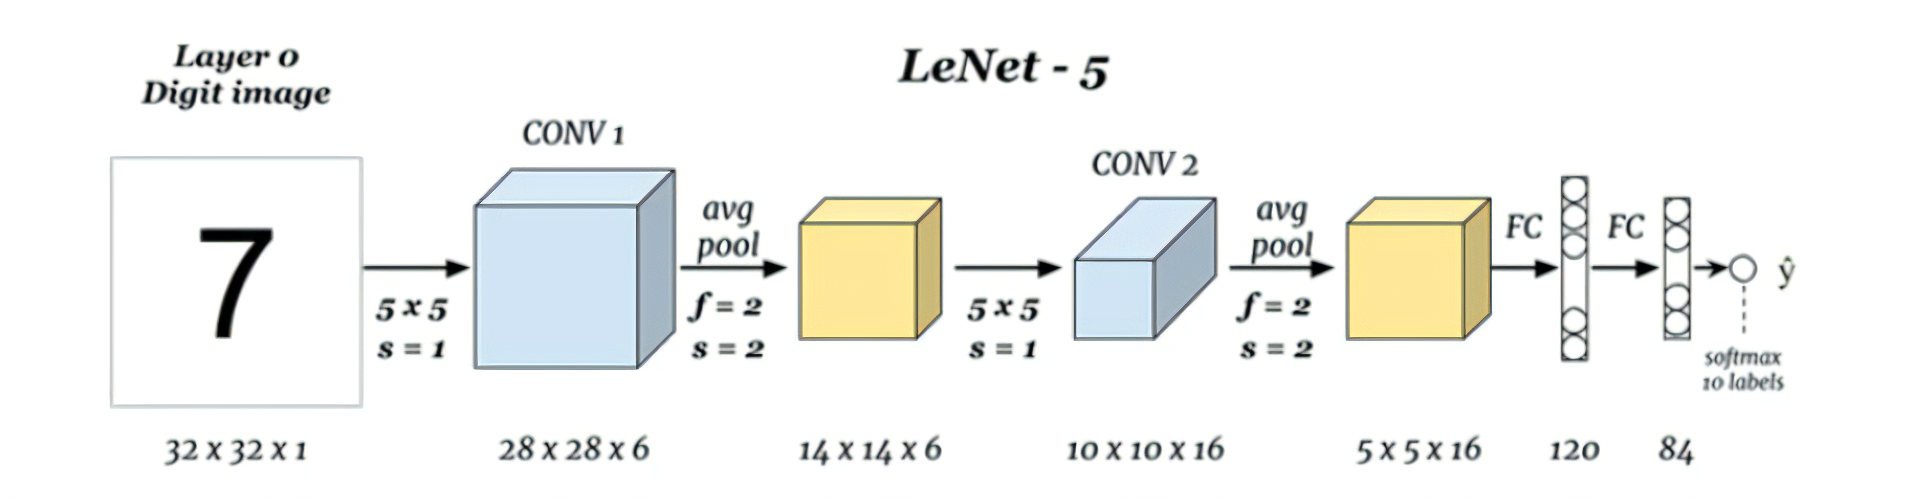
\includegraphics[width=.9\textwidth]{figures/ann/LeNetx2.png}
    \caption{LeNet's 5 Architecture.}
    \label{fig:leNet}
\end{figure}
LeNet-5, developed by Yann LeCun and his colleagues in the late 1990s\cite{lecunGradientbasedLearningApplied1998},
is widely regarded as the pioneer of modern Convolutional Neural Networks. Designed primarily for handwritten digit
recognition, specifically the MNIST dataset, LeNet-5 laid the foundation for subsequent advancements in deep learning.
The architecture consists of two sets of convolutional and subsampling layers, followed by three
fully connected layers. Observing \cref{fig:leNet}, the original LeNet architecture utilized average pooling,
that was a standard of the era, yet with current knowledge max pooling layers would be preffered, producing
slightly improved results. However, for this analysis the vanilla version, as introduced in the original papar,
is showcased.


The simple yet effective design of \emph{LeNet-5} demonstrated the potential of CNNs in automatically learning hierarchical features
from raw pixel data, a concept that has been fundamental to later architectures. LeNet's success in recognizing handwritten digits
was revolutionary for its era, and is still regarded as one of the most important historically CNN architectures.

% \subsection{AlexNet}
% \begin{figure}[!ht]
%     \centering
%     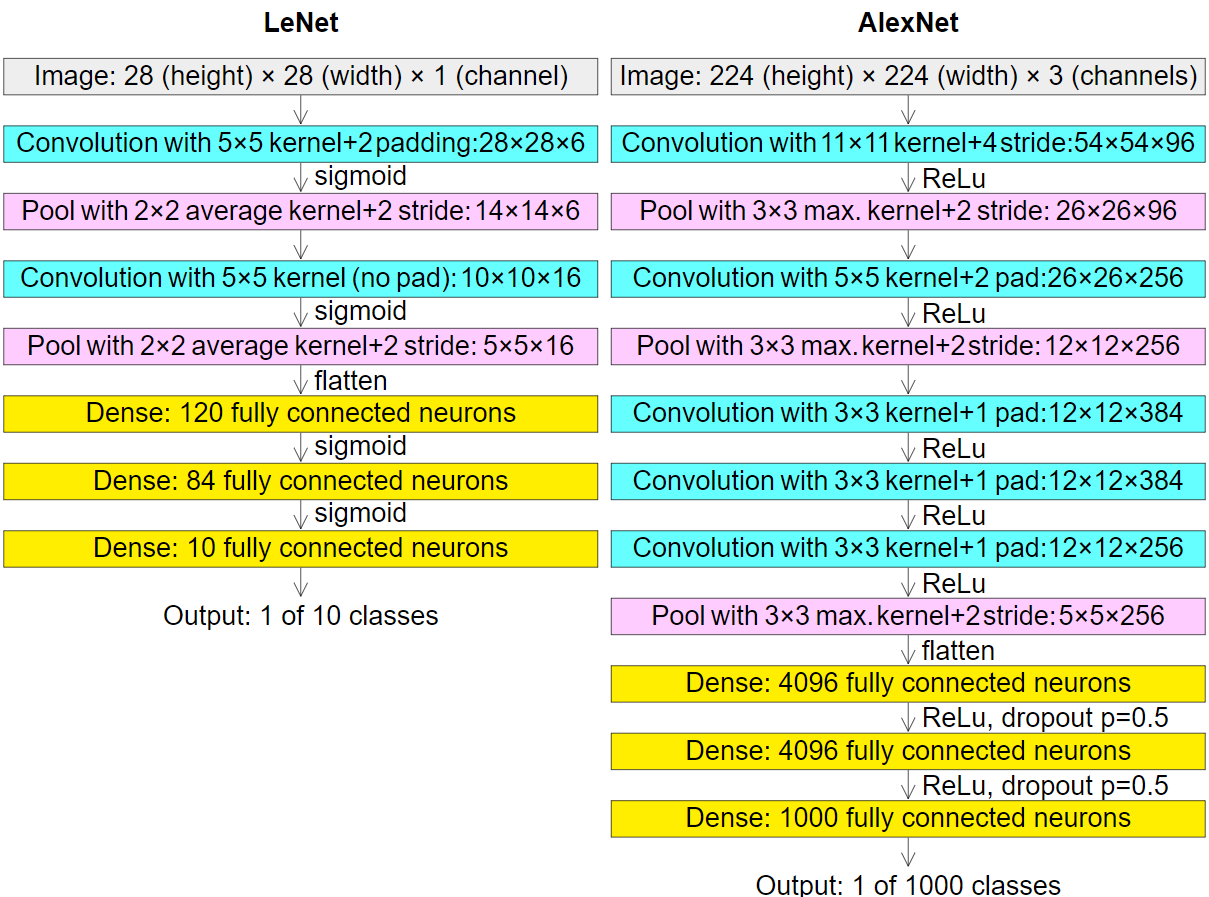
\includegraphics[height=.55\textwidth,keepaspectratio]{figures/ann/AlexNet.png}
%     \caption{A comparison between LeNets and the evolution of AlexNet.}
%     \label{fig:alex_net}
% \end{figure}


% Introduced by Alex Krizhevsky et al.\ in 2012\cite{krizhevskyImageNetClassificationDeep2012}, AlexNet marked a significant breakthrough in the field of deep learning and computer vision,
% by winning the ILSVRC in 2012, by a large margin. AlexNet's architecture is a significant evolution from LeNet-5, being both larger and deeper, yet sharing principal similarites.
% A direct comparison to \emph{LeNet} is depicted in \cref{fig:alex_net}.
% As illustrated, AlexNet involves five convolutional layers, some followed by max-pooling layers, and three fully connected layers. This implementation
% It introduced several key innovations that have become standard in modern CNNs.



% Unlike LeNet-5, which alternates between convolutional and pooling layers, AlexNet stacks multiple convolutional
% layers directly on top of each other before applying pooling, allowing the network to learn more complex features at each level.
% Additionally, AlexNet, also, popularized the use of ReLUs as activation functions, significantly speeding up the training process compared
% to traditional activation functions like sigmoid or tanh. While the idea of using GPUs for machine learning was explored prior to AlexNet,
% this model effectively demonstrated the power of GPU acceleration in training deep neural networks, utilizing two GPUs to handle the
% computational demands of the large ImageNet dataset. To address the problem of overfitting, AlexNet employed dropout layers, which
% randomly deactivate a subset of neurons during training, forcing the network to learn redundant representations and thereby improving generalization.

% Summing up AlexNet's success demonstrated the viability of deep learning for complex image classification tasks, sparking widespread
% interest and research in the field.
\subsection{VGG16}
\begin{figure}[!ht]
    \centering
    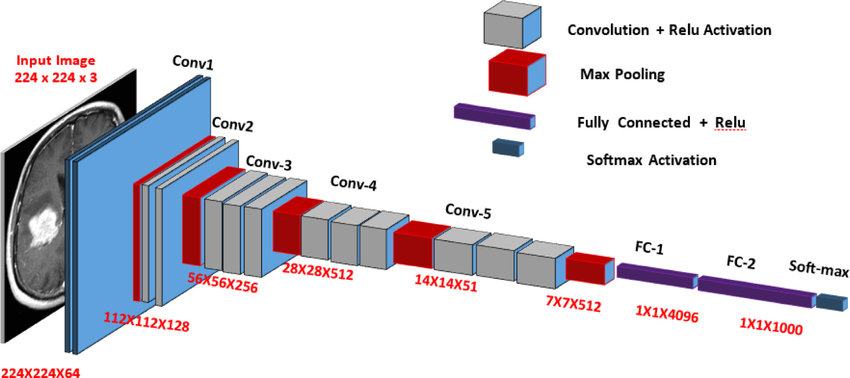
\includegraphics[width=.8\textwidth]{figures/ann/vgg16.png}
    \caption{VGG16 Architecture.}
    \label{fig:vgg16}
\end{figure}
VGG16, introduced by the Visual Geometry Group and specifically A. Zisserman and K. Simonyan from the University of Oxford\cite{simonyanVeryDeepConvolutional2015},
and based its implementation on the notion that the performance of a deep neural network can be improved by increasing the model's depth. To be precise, the number 16
on the ann's names was assigned for the 16 parameter layers that comprise the model, 13 of which are convolutional layers and the rest 3 arefully connected layers.
VGG16 is renowed for its simplicity and robust performance in a variety of computer vision tasks. Its architecrure comprises of stacked convolution layers
followed by max-poolinh layers, with progressively increasing depth.

The primary novelty of the model's architecture was that it mitigates the network's parameters by leveraging $3 \times 3$ kernels with a stride of 1 to replicate a kernel of any size.
In essence, the dimensions of the output of any convuled layer can be reached by stacking several smaller layers.
An example will be demonstrated to understand the above logic. Consider a $5 \times 5$ image that is convuled with a $5 \times 5$ kernel. This produces an output matrix of $1 \times 1$.
Let the same image be convuled by a $3 \times 3$ kernel, producing a $3 \times 3$ matrix that can be additionally convuled by another $3 \times 3$ kernel. The result will be an output
matrix of $1 \times 1$. In this example both processes reult on a $1 \times 1$ matrix, yet the single kernel required $5 \cdot 5= 25$ parameters while the two stacked
convolution layers required: $3 \cdot 3 + 3 \cdot 3 = 18$ parameters.

Following the innovative example of AlexNet-the 2012 ILSVRC winner- VGG16 employed ReLu activation functions in all the layers, reducing training time, while leveraging
SoftMax function in the output layer to normalize the probability of the classes.

Combining the aforementioned elements, this architecrure managed to classify with great precision images to 1000 object categories and became a significant paradigm in
the field of ConvNets, still being utilized in systems that conduct deep learning.


\subsection{ResNet}

\begin{figure}[!ht]
    \centering
    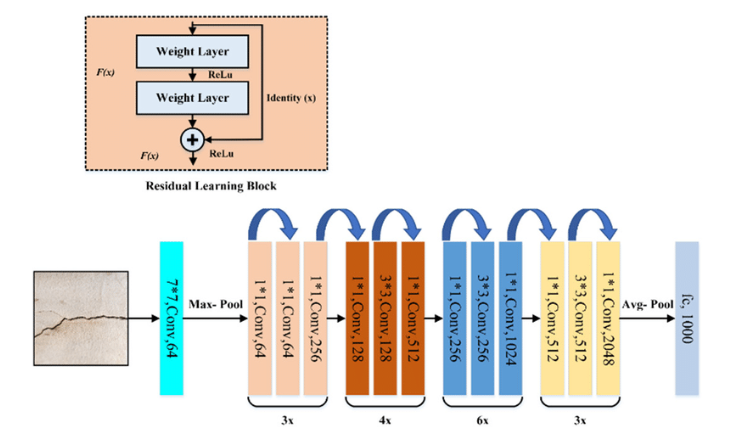
\includegraphics[width=.8\textwidth]{figures/ann/ResNet.png}
    \caption{ResNet's Architecture with residual learning block illustration.}
    \label{fig:res_net}
\end{figure}
Residual Networks (ResNet), introduced by Kaiming He et al.\ in 2015\cite{heDeepResidualLearning2015}, addressed the degradation problem in very deep
networks. ResNet's key innovation is the introduction of residual learning blocks, or shortcuts, which add the input of the block directly to its output,
allowing the network to learn identity mappings. These connections help prevent the vanishing gradient phenomenon during backpropagation and mitigate accuracy
saturation, enabling the effective training of much deeper networks compared to previous architectures.

ResNet variants, such as ResNet-50, ResNet-101, and ResNet-152, have achieved remarkable success, with ResNet-152 achieving a top-5 error rate of 3.57\% in the
ILSVRC 2015, setting new performance standards. The success of ResNet demonstrated that increasing network depth could lead to better performance, provided that
appropriate architectural adjustments are made to ensure effective training.

These architectures—LeNet, AlexNet, and ResNet—represent significant milestones in the evolution of CNNs, each contributing foundational ideas and techniques
that have driven the field forward.